\subsection{Overview of Mobile Application Development}
The evolution of mobile app development has seen significant advancements from early platforms to the modern ecosystems of Android and iOS. Initially, Java dominated Android development, offering a robust and versatile language for creating mobile applications. However, the introduction of Kotlin by JetBrains marked a pivotal moment in Android development. Kotlin, with its concise syntax, enhanced safety features, and seamless interoperability with Java, quickly gained popularity among developers. Google recognized the potential of Kotlin and endorsed it as a preferred language for Android app development, leading to widespread adoption within the Android community \cite{zhang2023entertainment}. Furthermore, the emergence of cross-platform frameworks like Flutter, developed by Google, has revolutionized mobile app development by enabling developers to write code once and deploy it across multiple platforms. Flutter allows for fast development, expressive UIs, and native performance, making it popular for developers aiming to create visually appealing and responsive applications.
\par
Choosing between native development and cross-platform frameworks is a strategic decision that goes beyond technical considerations and impacts the success of a mobile application. Native development offers optimized performance and better access to device-specific features, ensuring high user satisfaction. On the other hand, cross-platform frameworks provide advantages such as faster rollout and cost-effectiveness. The decision between these approaches has implications for app performance, maintainability, and overall user experience, making selecting the appropriate development approach crucial. Native development allows developers to leverage platform-specific features and functionalities, resulting in high-performance applications tailored to each operating system. In contrast, cross-platform frameworks enable developers to write code once and deploy it across multiple platforms, reducing development time and costs. The study emphasizes the importance of well-defined technical requirements and specifications in selecting a cross-platform framework or development approach \cite{biorn2020empirical}.
\par
Java and Kotlin have been long-standing choices for native Android app development, with Java being the traditional standard and Kotlin emerging as a modern alternative. Java, known for its robustness and extensive ecosystem, has been widely used for Android development \cite{wasilewski2021comparison}. In contrast, Flutter, utilizing Dart, has gained attention for its cross-platform capabilities, offering a single codebase for both Android and iOS platforms, simplifying development, and reducing maintenance costs \cite{prasetia2023development}. The comparative analysis of Java, Kotlin, and Flutter reveals distinct advantages and challenges associated with each technology. Java and Kotlin excel in native Android development, with Kotlin offering modern features and improved safety. On the other hand, Flutter stands out for its cross-platform capabilities, enabling developers to create applications for multiple platforms with a single codebase \cite{Meiller_2022}.
\par
The quality of code is a vital component of software development, as it has a significant impact on the performance, scalability, and maintainability of applications. Key indicators of code quality include identifying code smells, which are patterns in the code that may indicate potential issues, and assessing the overall complexity of the codebase. Although code smells may not immediately affect the program's functionality, they can increase the risk of bugs or failures down the line and make maintenance more complex \cite{banker1998software}.
\par
Despite the critical role of mobile applications in various sectors and the rapid evolution of development technologies, there remains a significant gap in empirical research regarding the comparative analysis of mobile development approaches, particularly regarding their impact on code quality. Most existing studies focus on individual aspects of development, such as usability, performance, or developer preferences. Still, few comprehensively evaluate how different programming languages and frameworks—like Java, Kotlin, and Flutter—affect code's overall quality and maintainability. Current literature extensively discusses the features and benefits of Kotlin and Flutter, noting their potential to streamline the development process and enhance code safety and maintainability. However, more systematic empirical studies need to quantify the impact of these modern languages and frameworks on code quality in real-world development scenarios. This includes a detailed analysis of code smells, which are subtle indicators of potential future problems or technical debt that might not currently affect an application's functionality but could lead to significant maintenance challenges. Furthermore, while tools like SonarQube offer capabilities to assess and compare code quality metrics across different environments, the practical application of these tools in comparative studies must be extensively documented in academic research. Studies that not only use these tools to gather data but also critically analyze this data to provide actionable insights into how specific characteristics of Java, Kotlin, and Flutter influence the maintainability, scalability, and efficiency of the development process are needed.
\par
This research aims to fill these gaps by conducting a rigorous comparative analysis of mobile applications developed in Java, Kotlin, and Flutter. It will evaluate various code quality metrics, such as the prevalence and severity of code smells and the overall complexity of the codebases, to determine the tangible impacts of choosing one technology over another. This study will provide empirical evidence to guide developers in selecting the most suitable programming language or framework for their projects based on quantifiable code quality and maintainability measures. By addressing this research gap, the study will contribute valuable insights to the field of software engineering, particularly mobile app development. It will enhance understanding of the practical implications of development tool choices on long-term application success and sustainability.
\subsection{Study Objectives and Research Questions}
The overarching objective of this thesis is to conduct a thorough empirical analysis to compare the impact of different mobile development approaches—specifically Java, Kotlin, and Flutter—on the quality and maintainability of mobile applications. This research is driven by the need to provide developers and stakeholders with data-driven insights that can guide their decisions regarding which development technologies to adopt, depending on specific project requirements and goals. 
\par
The choice of focusing on these specific technologies is substantiated by their prevalent use and perceived benefits within the development community. According to a 2022 developer survey, Flutter has emerged as the most popular cross-platform mobile framework. The survey reports that 46 percent of software developers used Flutter, highlighting its significant adoption. This statistic is particularly compelling, considering that approximately one-third of mobile developers utilize cross-platform technologies, while the remainder prefer native tools.
\begin{figure}[htbp]
    \centering
    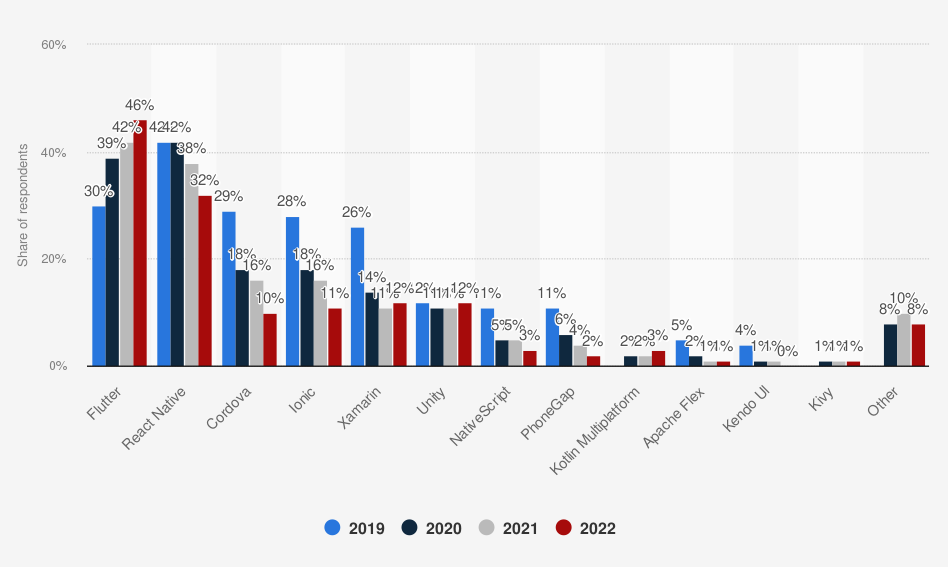
\includegraphics[scale = 0.45]{img/cross_platform-sts.png}
    \caption{Cross-platform mobile frameworks used by software developers worldwide from 2019 to 2022 \cite{jetbrains2022}}
    \label{fig:cross_platform-sts}
\end{figure}
\subsubsection*{Objectives}
\begin{enumerate}
    \item To evaluate the development efficiency of Java, Kotlin, and Dart. This includes measuring the time taken for development, the ease of implementation of features, and the integration of third-party services across the three languages.
    \item To analyze the code quality of Java, Kotlin, and Dart applications. Code quality will be assessed by examining code complexity, readability, and the ability to adapt or extend the application with new features.
    \item This study aims to compare the code quality of applications developed using Java, Kotlin, and Dart(Flutter). Code quality will be evaluated based on the prevalence of code smells, adherence to coding standards, and the occurrence of bugs or issues during and after development.
    \item To provide recommendations on the choice of development approach based on empirical data: Based on the findings, the study aims to offer guidelines on selecting development approaches for different mobile app projects, considering factors like project size, complexity, and specific industry needs.
\end{enumerate}
\subsubsection*{Research Questions}
In pursuit of these objectives, the study will seek to answer the following research questions:
\begin{enumerate}
    \item Comparing the Efficiency and Resource Utilization of Java, Kotlin, and Dart: How does each technology stack up against one another regarding development efficiency, time, and resources required to create a fully operational mobile application? What are the implications of selecting each technology for the development process?
    \item Considering the Impact on Long-Term Code Quality: What are the consequences of choosing Java, Kotlin, or Dart on mobile application code quality? How do code complexity, debugging ease, and change adaptability impact long-term code quality in these development environments?
    \item Navigating Coding Challenges and Selection Criteria: How does each development approach—Java, Kotlin, or Dart—address prevalent coding challenges and quality issues, such as the frequency and severity of code smells? Based on these considerations, which development approach is most desirable for various mobile application projects? Considering project scope, performance requirements, and target platforms, what are the recommendations for language selection to optimize development outcomes?
\end{enumerate}
\subsection{Methodology, Significance, and Structure of Thesis}
A robust methodology has been adopted to achieve the research objectives outlined in this study, which involves developing a Kanban board application using three distinct programming environments: Java, Kotlin, and Flutter. The subsequent analysis of these applications will employ SonarQube, a sophisticated tool designed to assess metrics such as lines of code (LOC), code smells, and overall code quality. This method not only facilitates the collection of quantitative data concerning the efficiency and maintainability of each language but also provides qualitative insights into the coding experience. Such a dual-focused analysis enables a comprehensive understanding of the practical impacts of each development approach on project outcomes.
\par
The insights derived from this research are expected to be highly valuable for developers and project managers, guiding the selection of development tools and practices based on empirical evidence. By clearly delineating the strengths and weaknesses associated with Java, Kotlin, and Flutter, this study contributes to informed decision-making within the software development community. Such knowledge is crucial for enhancing app quality and developer satisfaction, and it is anticipated that the findings will encourage more efficient and effective development practices within the industry. The practical implications of this research are significant, offering potential improvements in development processes, resource allocation, and project management in mobile app development.
\par
This thesis is methodically structured into six comprehensive chapters, designed to guide the reader through the research process systematically:

\begin{itemize}
    \item \textbf{Introduction:} This opening chapter sets the stage by outlining the motivation for the study, the research gaps identified, and the objectives to be achieved.
    \item \textbf{Literature Review:} This section delves into a thorough review of existing research, discussing the theoretical frameworks and previous empirical studies relevant to mobile application development, mainly focusing on Java, Kotlin, and Dart(Flutter).
    \item \textbf{Methodology:} This section details the specific methods employed in the study, including the development processes for the Kanban board application in each programming environment and the analytical tools and criteria used to evaluate code quality. 
    \item \textbf{Results:} This paper presents a detailed account of the application development and analysis findings, offering a comparative perspective on the code quality metrics observed across the different programming environments.
    \item \textbf{Discussion:} This section interprets the results in the context of existing literature and discusses their implications for developers and the broader software development industry.
    \item \textbf{Conclusion and Recommendations:} This section summarizes the findings, discusses the study’s potential limitations, and offers recommendations for future research and practical applications in mobile app development.
\end{itemize}
